\documentclass[11pt]{article}
%\usepackage[titlepage]{polytechnique}
\usepackage[utf8]{inputenc}     
\usepackage{amsmath}
\usepackage{amssymb}
\usepackage{amsfonts}
\usepackage[francais]{babel}
\usepackage[version=3]{mhchem}
\usepackage{epstopdf}
\usepackage[justification=centering]{caption}
\usepackage{slashbox}
\usepackage[T1]{fontenc}
\usepackage{tikz}
\usetikzlibrary{arrows} 
\usepackage{pgfplots}
%\usepackage[hidelinks,hyperfootnotes=false]{hyperref}
\usepackage{subcaption}
\usepackage{amsthm}
\usepackage{empheq}

\usepackage{geometry}

\newcommand*\widefbox[1]{\fbox{\hspace{2em}#1\hspace{2em}}}
\theoremstyle{definition}

\newtheorem{definition}{Definition}[section]

\theoremstyle{remark}
\newtheorem*{remark}{Remark}


%\title{Notes for Seance 2}
\title{On Brownian Motion, Ito Calculus and the Feynman-Kac Formula}


\begin{document} 
\maketitle 

Dans cette partie nous décrirons une méthode probabiliste pour évaluer le noyau $k_{\beta}$ que nous avons décrit dans la section précédente. 
Avant de commencer le calcul de $k_{\beta}$, nous allons introduire quelques notions utiles.

\section{Definitions}

\theoremstyle{definition}

\begin{definition}{\textbf{Processus de Markov}}

Soit $(X_n)_{n >0}$ un processus aléatoire discret sur un espace d'états dénombrable $E$. Le processuss satisfait la propriété de Markov si pour toute collection d'états $(x_0, x_1, ... x_n) \in E$, nous avons 

\begin{equation} 
\mathbb{P}(X_{n+1} = y | X_0 = x_0, X_1 = x_1,....X_n = x_n) = \mathbb{P}(X_{n+1} = y | X_n = x_n)
\end{equation}

Il faut que les deux probabilités conditionnelles soient bien définies. Le processus $(X_n)_{n>0} $ est alors appelé un processus de Markov.

\end{definition}

\begin{definition}{\textbf{Ergodicité}}

Un processus est ergodique s'il satisfait les conditions suivantes :

\begin{itemize}

\item 

$\varphi$ est une mesure de probabilité invariante par le processus de Markov. 

\item 

\textbf{Condition d'accessibilité}: 

\begin{align}
\forall \mathrm{B} \in \mathcal{B}(\mathbb{R}^d)\quad \mathrm{t.q.}\quad \varphi(\mathrm{B})>0, \quad \forall x\in\mathbb{R}^d, \quad \exists n\in\mathbb{N} \quad \mathrm{t.q.}\quad \mathbb{P}(\mathrm{X}_n \in \mathcal{B} | \mathrm{X}_0 =n ) > 0 
\end{align}
\end{itemize}

\end{definition}

\begin{remark}
\begin{enumerate}
\item 
Nous avons défini la notion d'ergodicité sur $\mathbb{R}^d$, mais les mêmes définitions restent valables pour $\mathrm{L}\mathbb{T}^d$.
\item 
Au moment de simuler avec l'algorithme de Metropolis, il suffira de vérifier que la probabilité de transfert pour cet algorithme satisfait la condition d'accessibilité dans la définition d'ergodicité.

\end{enumerate}
\end{remark}


\begin{definition}{\textbf{Chaînes de Markov}}

Une chaîne de Markov (discrète) est un processus de Markov défini par :

\begin{equation}
\left\{ 
  \begin{array}{ll}
  \mathrm{X}_{n+1}^{\Delta t} &= \mathrm{X}_{n}^{\Delta t} + b(\mathrm{X}_{n}^{\Delta t}) + \sqrt{\Delta t} \xi_{n}
  \\
  \mathrm{X}_{0}^{\Delta t} &\sim  f(x) \mathrm{d}x 
  \end{array}
\right.
\end{equation}



avec $x \in \mathbb{R}^d$ et $b: \mathbb{R}^d \to \mathbb{R}^d$ une fonction régulière. Ici $\xi_{j} \sim \mathcal{N}(0,1)_{\mathbb{R}^d}$, i.e. $\xi_{j}$ est un vecteur gaussien de dimension $d$. 
\end{definition}

À partir de la chaine de Markov defini ci-dessus nous pouvons construire un processus de Markov en temps continu en reliant les instants de temps $t_n$ et $t_{n+1}$ de manière affine. Dans ce cas, nous avons avec les mêmes conditions que ci-dessus :

\begin{align}
\forall t \in [t_n,t_{n+1}],\quad\tilde{\mathrm{X}}_{t}^{\Delta t} &= \mathrm{X}_{n}^{\Delta t} + (t-t_n) \mathrm{X}_{n+1}^{\Delta t} 
\end{align}

Nous avons de même 
\begin{equation}
\tilde{\mathrm{X}}_{t}^{\Delta t} \underset{\Delta t \to 0}{\longrightarrow} \mathrm{X}_t
\end{equation}


où $\mathrm{X}_{t}$ suit l’équation différentielle stochastique donnée par: 

\begin{align}
\label{equ_stoch_x}
\mathrm{dX}_{t} &= b(\mathrm{X}_{t})\mathrm{d}t + \mathrm{dW}_{t} \\
\mathrm{X}_{0} &\sim f(x)\mathrm{d}x
\end{align}

où $\mathrm{W}_{t}$ est le processus de Wiener.

\section{Formule d'Itô}

A la fin de la section précédente, nous avons abouti à une équation différentielle stochastique qui détermine le processus de Markov en temps continu. Pour faciliter la résolution de cette équation, nous  mettrons en place des formules de calcul différentiel stochastique qui nous permettront d'aboutir à la formule de Feynman-Kac. 

Considérons d'abord l’équation \eqref{equ_stoch_x} sans le terme stochastique $\mathrm{dW}_{t}$. Dans ce cas, l'équation devient déterministe et sa solution $\mathrm{Y}_t$ suit l'équation:

\begin{equation}
\frac{\mathrm{dY}_{t}}{\mathrm{d}t} = b(\mathrm{Y}_t) 
\end{equation}

Pour rester dans un cadre simple, nous travaillerons dans $\mathbb{R}$, mais les résultats sont bien évidemment généralisables sur $\mathbb{R}^d$. Soit $h: t \times \mathbb{R}^d \rightarrow \mathbb{R}$. Alors nous avons : 

\begin{align*}
\mathrm{d}(h(\mathrm{Y}_{t})) &= \frac{\partial h}{\partial t}(t,\mathrm{Y}(t)) \mathrm{d}t + \nabla h(\mathrm{Y}_{t}) \mathrm{dY}_{t} \\
&= \frac{\partial h}{\partial t}(t,\mathrm{Y}(t)) \mathrm{d}t + \nabla h(\mathrm{Y}_{t}) b(\mathrm{Y}_{t})\mathrm{d}t
\end{align*}

Dans le cas de $\mathrm{X}_{t}$, solution de l'équation différentielle stochastique \eqref{equ_stoch_x}, la différentielle de $h(t, \mathrm{X}_t)$ contient un terme supplémentaire faisant intervenir les dérivées secondes de h. Nous obtenons finalement:

\begin{equation}
\mathrm{d}(h(t,\mathrm{X}_t)) = ( \frac{\partial h}{\partial t}(t, \mathrm{X}_t) + \nabla h(t,\mathrm{X}_t) b(\mathrm{X}_t) + \frac{1}{2} \Delta h(t,\mathrm{X}_t) )\mathrm{d}t + \nabla h(t,\mathrm{X}_t) \mathrm{dW}_{t}
\end{equation}

\section{Le Formule de Feynman-Kac}

Munis des règles du calcul différentiel, nous sommes maintenant en mesure de dériver la formule de Feynman-Kac.

Pour ce faire, nous introduisons deux équations : les équations de Kolmogorov forward et backward 

\begin{definition}{\textbf{L'equation de Kolmogorov forward}}
C'est une équation différentielle associé à \eqref{equ_stoch_x} définie  dans $]0,\beta] \times \Omega$par : 

%Il faut expliciter le domaine, j'imagine ? Ou la classe de u ? 
\begin{equation}
\label{kolmo_forw}
\begin{split}
\frac{\partial u}{\partial t} &= \frac{1}{2} \Delta u - \mathrm{div}(bu) - \mathrm{V}u \\
u(0) &= f(x)
\end{split}
\end{equation}

\end{definition}



\begin{definition}{\textbf{L'équation de Kolmogorov backward}}

Dans $]0,\beta] \times \Omega$, nous definissons l'equation de Kolmogorov backward associé à \eqref{equ_stoch_x}

\begin{equation}
\label{kolmo_back}
\begin{split}
\frac{\partial v}{\partial t} + \frac{1}{2} \Delta v + b \nabla v - \mathrm{V}v &= 0 \\
v(\beta, x) &= g(x)
\end{split}
\end{equation}
\end{definition}

Nous considérons la dérivée totale $\mathrm{d}(v(t, \mathrm{X}_{t}) e^{-\int_0^{t} \mathrm{V}(\mathrm{X}_{s}) \mathrm{d}s})$ où $\mathrm{X}_{t}$ est défini en \eqref{define_xt}. En utilisant l'équation \eqref{develop_ito_x}, nous trouvons que :

\begin{multline}
\begin{split}
\mathrm{d}(v(t, \mathrm{X}_{t}) e^{-\int_0^{t} \mathrm{V}(\mathrm{X}_{s}) \mathrm{d}s}) = (\frac{\partial v}{\partial t} + b \nabla v + \frac{1}{2}\Delta v - \mathrm{V}v)e^{-\int_0^{t} \mathrm{V}(\mathrm{X}_{s}) \mathrm{d}s} \\
+ \nabla v(t, \mathrm{X}_t)\mathrm{dW}_{t} e^{-\int_0^{t} \mathrm{V}(\mathrm{X}_{s}) \mathrm{d}s}
\end{split}
\end{multline}

et le premier terme est nul d'après \eqref{kolmo_back}. Donc :

\begin{align}
\mathrm{d}(v(t, \mathrm{X}_{t}) e^{-\int_0^{t} \mathrm{V}(\mathrm{X}_{s}) \mathrm{d}s}) = \nabla v(t, \mathrm{X}_t)\mathrm{dW}_{t} e^{-\int_0^{t} \mathrm{V}(\mathrm{X}_{s}) \mathrm{d}s}
\end{align}

Enfin nous remarquons que l’espérance de $\nabla v(t, \mathrm{X}_t)\mathrm{dW}_{t} e^{-\int_0^{t} \mathrm{V}(\mathrm{X}_{s}) \mathrm{d}s}$ est nulle, et en utilisant la commutation des différentes opérations avec l’espérance, nous avons ainsi que: 

\begin{align}
\mathbb{E}(v(t , \mathrm{X}_{t})e^{-\int_0^{t} \mathrm{V}(\mathrm{X}_{s}}) = \mathrm{cte}
\end{align}

En particulier:

\begin{align}
\mathbb{E}(v(\beta , \mathrm{X}_{\beta})e^{-\int_0^{\beta} \mathrm{V}(\mathrm{X}_{s})}) &= \mathbb{E}(v(0, \mathrm{X}_0)), \\
\mathbb{E}(g(x_{\beta}))e^{-\int_0^{\beta} \mathrm{V}(\mathrm{X}_{s})}) &= \int_{\Omega} v(0,x) f(x) \mathrm{d}x.
\end{align}

où nous avons utilisé la condition initiale de \eqref{kolmo_back} et où l’intégration porte sur l'ouvert $\Omega$ considéré. 

Considérons maintenant l'intégrale $\int_{\Omega} v(0,x) f(x) \mathrm{d}x$. Par la condition initiale de \eqref{kolmo_forw}, nous avons par conséquent :

\begin{equation}
\int_{\Omega} v(0,x) f(x) \mathrm{d}x = \int_{\Omega} v(0,x) u(0,x) \mathrm{d}x
\end{equation}

D'où:

\begin{align}
\label{expansion_integral_vu}
\begin{split}
\int_{\Omega} v(0,x) u(0,x) \mathrm{d}x &= \int_{\Omega} v(\beta, x) u(\beta,x) \mathrm{d}x - \int_{0}^{\beta} \frac{\mathrm{d}}{\mathrm{d}t}\left(\int_{\Omega} v(t,x) u(t,x) \mathrm{d}x \right) \mathrm{d}t \\
&= \int_{\Omega} v(\beta, x) u(\beta,x) \mathrm{d}x - \int_{0}^{\beta} \left( \int_{\Omega} \frac{\partial v}{\partial t} u \mathrm{d}x + \frac{\partial u}{\partial v} \mathrm{d}x \right) \mathrm{d}t
\end{split}
\end{align}

Nous remarquons alors que les problèmes \eqref{kolmo_forw} et \eqref{kolmo_back} sont l'adjoint l'un de l'autre pour le produit scalaire usuelle defini pour l'espace $\mathrm{L}^2$. En d'autres termes, si $L$ est un opérateur différentiel et $L^{*}$ son opérateur adjoint, nous avons : 

\begin{align}
\label{adjoint_conditions}
\begin{split}
\frac{\partial u}{\partial t} &= \mathrm{L}u  \\
\frac{\partial v}{\partial t} &= -\mathrm{L}^{*}v
\end{split}
\end{align}

En d'autres termes :
\begin{align}
- \int_{0}^{\beta} \left( \int_{\Omega} \frac{\partial v}{\partial t} u \mathrm{d}x + \frac{\partial u}{\partial v} \mathrm{d}x \right) \mathrm{d}t &= 
- \int_{0}^{\beta} \left( (-L^{*}v,u)_{\mathrm{L}^2} + (v, Lu)_{L^2} \right) \mathrm{d}t &= 0
\end{align}

Ainsi :

\begin{align*}
\int_{\Omega} v(\beta, x) u(\beta, x) \mathrm{d}x &= \int_{\Omega} v(0,x) f(x) \mathrm{d}x \\
\int_{\Omega} g(x) u(\beta, x) \mathrm{d}x &= \int_{\Omega} v(0,x) f(x) \mathrm{d}x
\end{align*}

et on déduit la formule de Feynman-Kac : 

\begin{empheq}[box=\widefbox]{align}
\label{feynman_kac}
\int_{\Omega} g(x) u(\beta,x) \mathrm{d}x &= \mathbb{E}\left( g(x_{\beta}) e^{-\int_{0}^{\beta} \mathrm{V}(x_s)\mathrm{d}s} \right)
\end{empheq}

où $\mathrm{X}_{t}$ est la solution de \eqref{equ_stoch_x}

\section{Application à notre problème} 

Revenons sur notre problème de départ, qui est de trouver le noyau de l'opérateur $e^{-\beta H}$. Nous rappelons que le noyau est une fonction $k_{\beta}$ telle que:

\begin{equation}
\label{def_noyau} 
\left(e^{-\beta H} f \right)(x) = \int_{\Omega} k_{\beta}(x,y) f(y) \mathrm{d}y
\end{equation}

Nous remarquons que, pour $b=0$, $e^{-\beta H} f$ est la solution de \eqref{kolmo_forw}. D'où en appliquant \eqref{feynman_kac} :

\begin{equation}
\int_{\Omega X \Omega} k_{\beta}(x,y) f(y)g(x) \mathrm{d}x\mathrm{d}y = \mathbb{E}\left( g(\mathrm{X}_{\beta}) e^{-\int_{0}^{\beta} \mathrm{V}(\mathrm{X}_s)\mathrm{d}s} \right)
\end{equation}

où $\mathrm{X}_t$ est la solution de \eqref{equ_stoch_x}. 

Cette dernière condition étant vraie pour tout $f$, nous prenons $f(y) = \delta(y)$, le delta de Dirac. Dans ce cas, nous avons pour le processus $\mathrm{X}_{t}$ : 
\begin{equation}
\mathrm{X}_{\beta} = y + \mathrm{W}_{\beta}
\end{equation}. 

D'où:

\begin{align}
\begin{split}
\int_{\Omega} k_{\beta}(x,y) g(x) \mathrm{d}x &= \mathbb{E}\left( g(y+\mathrm{W}_{\beta}) e^{-\int_{0}^{\beta} V(y+\mathrm{W}_s) \mathrm{d}s} \right) \\
&= \int_{\Omega} g(x) \mathbb{E}_{y+\mathrm{W}_{\beta}=x} \left( e^{-\int_{0}^{\beta} V(y+\mathrm{W}_{s}) \mathrm{d}s} \right) \mathrm{d}x
\end{split}
\end{align}

Nous identifions alors le noyau comme étant : 

\begin{empheq}[box=\widefbox]{align}
\label{noyau_esperance}
k_{\beta}(x,y) = \mathbb{E}_{y+\mathrm{W}_{\beta}=x} \left( e^{-\int_{0}^{\beta} V(y+\mathrm{W}_{s}) \mathrm{d}s} \right)
\end{empheq}

Dans notre cas, nous nous intéressons au calcul de la fonction de partition $Z = \mathrm{Tr}(e^{-\beta H})$, qui d'après ce qui précède s'écrit : 

\begin{align}
\label{partition_func_martingale}
\begin{split}
Z &= \mathrm{Tr}(e^{-\beta H}) = \int_{\Omega} k_{\beta}(x,x) \mathrm{d}x \\
&= \int_{\Omega} \mathbb{E}_{\mathrm{W}_{\beta} =0} \left( e^{-\int_{0}^{\beta} V(x+\mathrm{W}_{s})} \right)
\end{split}
\end{align}

\begin{remark}
Nous devons interpréter les deux termes dans cette dernière relation. Prenons d'abord $\mathbb{E}_{\mathrm{W}_{\beta=0}}$. C'est le terme d’espérance sur les ponts browniens, c'est-à-dire une espérance sur tous les chemins allant de $x_0$ au temps $t=0$ jusqu'au un temps $\beta$ où l'on revient au point de départ $x_{\beta}=x_0$. 

Le deuxième terme en exponentiel représente la création ou annihilation des particules à un point $x+\mathrm{W}_{s}$ donné. Nous formons donc une image de ce processus comme suivant : 

\begin{enumerate} 

\item 

Le particule commence son trajet à $x_{t=0}=x_0 = 0$. Nous allons regarder seulement les trajets qui finissent à un temps $t=\beta$, de sorte que $x_\beta = 0$.

\item 

Pendant ce trajet, la particule peut être détruite ou créée selon le poids probabiliste $e^{-\int_{0}^{\beta} V(x+\mathrm{W}_{s})}$. 

\item 

L’espérance sur tous ces trajets nous donne la fonction de partition $Z = \mathrm{Tr}(e^{-\beta H})$. 
\end{enumerate}


\end{remark}


\section{Methodes numeriques}

Dans cette partie nous allons décrire les méthodes numériques utilisés afin de simuler les systèmes bosoniques. Mais avant de parler des méthodes numériques, nous allons décrire, en quelques mots, les systèmes bosoniques. 

\subsection{Systemes Bosoniques} 

Les systèmes bosoniques sont des systèmes constitué par des bosons. Les bosons, en mécanique quantique, sont des particules portant un nombre quantique dit "nombre quantique de spin" (ou \emph{Spin Quantum Number}) et ce nombre est toujours un entier. Dans la nature, il existe d'autres particules qui portent un spin qui est toujours un demi-entier: ceux sont des bosons. La différence entre les spins de bosons et fermions engendrent des grandes differences dans les comportements des systèmes constitués par des nombreuses particules de même type. 

En mécanique quantique, l'état de chaque système est gouverné par un état $|\psi \rangle$, qui contient toute l'information du système. Cet état évolue selon la fameuse équation de Schroedinger. Le fait que les bosons ont un spin entier et les fermions un spin demi entier a des implication sur les propriétés de l'état $| \psi \rangle$. En particulier, l’état décrivant un système de $N$ bosons est symétrique par échange de deux bosons tandis que l'état est antisymétrique pour des fermions. C'est-à-dire que pour un système comprenant $N$ bosons ou $N$ fermions, nous avons les relations suivantes: 

\begin{align} 
\label{symetrie_boson_fermion}
|n_1 n_2 \cdots n_N; B\rangle &= \sqrt{\frac{\prod_n m_n!}{N!}} \sum_p |n_{p(1)}\rangle |n_{p(2)}\rangle \cdots |n_{p(N)}\rangle \\
|n_1 n_2 \cdots n_N; F\rangle &= \frac{1}{\sqrt{N!}} \sum_p \operatorname{sgn}(p) |n_{p(1)}\rangle |n_{p(2)}\rangle \cdots |n_{p(N)}\rangle
\end{align}

où $B$ est pour les bosons, $F$ pour les fermions. Ici la somme porte sur touts les états possible sous une permutation $p$ de $N$ particules. La racine est pris afin de normaliser l'état. Finalement, $\operatorname{sgn}(p)$ est la signe de la permutation $p$ (+1 si $p$ contient un nombre paire des transpositions et -1 sinon). 

Vu qu'un état complet d'un système bosonique contient tous les permutations possible de $N$ particules, nous devons prendre en compte cette symétrie dans notre modélisation des systèmes bosoniques par un intégral de chemin. Concrètement, cela implique que pour un système des bosons, la matrice de densité est écrit de la manière suivante: 

\begin{align} 
\label{densite_boson}
\rho_{B}( \mathbf{R}, \mathbf{R}'; \beta) = \frac{1}{N!}\sum_{\mathcal{P}} \rho_{\mathrm{D}} (\mathbf{R}, \mathcal{P} \mathbf{R}'; \beta)
\end{align}

où $\rho_{\mathrm{D}}$ est la matrice de densité pour un système de $N$ particules distinguables. Pour les particules distinguables comme les particules classiques, nous pouvons commencer à un ensemble des points $\mathbf{R}$ donné et retourner à ce même point. Cependant, pour les particules comme des bosons(ou des fermions), nous pouvons arriver à un point $\mathcal{P}\mathbf{R}$, c'est-à-dire une permutation d'ensemble $\mathbf{R}$. Donc, en effectuant un calcul d’intégrale de chemin pour un système bosonique, nous devons sommer pas seulement sur tous les chemins allant de point $\mathbf{R}$ à $\mathbf{R}'$, mais sur tous les chemins partant de $\mathbf{R}$ et aboutissant à $\mathcal{P}\mathbf{R}'$. Cela fait à la fois la richesse dans le comportement des bosons mais aussi un problème technique dont nous devons faire face. 

\subsection{L'algorithme de Metropolis}

Un outil indispensable pour toutes les méthodes de Monte-Carlo est l'algorithme de Metropolis que nous allons décrire ici. 

L'algorithme de Metropolis est une méthode qui nous permet d'échantillonner une distribution de probabilité $P(\mathbf{X})$ dans les cas où l’échantillonnage direct est difficile. En particulier, nous pouvons utiliser cet algorithme si nous connaissons la distribution de probabilité à une constante multiplicative près. Dans le cas de la physique statistique, et par extension pour notre cas, cela nous permet de contourner le calcul de la fonction de partition (une quantité souvent difficile à calculer sauf dans des cas simples) et échantillonner selon une loi de probabilité (souvent la distribution de Boltzmann).

Concrètement, l'algorithme de Metropolis utilise une chaîne de Markov qui atteint assymptotiquement une distribution de probabilité $\pi(x)$ telle que $\pi(x) = P(x)$ où $P(x)$ est la distribution de probabilité souhaitée. L'algorithme de Metropolis construit une chaîne de Markov qui satisfait les conditions d'ergodicité et la condition d'existence d'une distribution stationnaire asymptotique. La condition d'existence d'une distribution stationnaire est écrit comme une équation de "bilan détaillé" :

\begin{equation}
\label{detailed_balance}
\pi(x) P(x \rightarrow x') = \pi(x') P(x' \rightarrow x)
\end{equation} 

où $\pi(x)$ est la distribution stationnaire et $P(x \rightarrow x')$ est la probabilité de passage de l'état $x$ à l'état $x'$ pour la chaine de Markov.  

Si la distribution stationnaire $\pi(x)$ est égale à $P(x)$, nous pouvons déduire la probabilité de passage entre deux états pour la chaine de Markov comme suit: 

\begin{enumerate} 
\item 
Nous écrivons 

\begin{align}
\label{derive_1}
P(x) P(x \rightarrow x') &= P(x') P(x' \rightarrow x) \\
\frac{P(x \rightarrow x')}{P(x' \rightarrow x)} &= \frac{P(x')}{P(x)}
\end{align} 

\item 
 
Ensuite, nous décomposons la probabilité de passage en deux parties: une probabilité dite de  "proposal" $g(x \rightarrow x')$, qui est la probabilité conditionnelle de proposer un état $x'$ étant donné un état $x$ et une probabilité d'acceptation $A(x \rightarrow x')$. Donc, la probabilité de passage s'écrit :

\begin{align} 
\label{derive_2}
P(x\rightarrow x') &= g(x\rightarrow x') A(x\rightarrow x') \\
\frac{A(x\rightarrow x')}{A(x'\rightarrow x)} &= \frac{P(x')}{P(x)}\frac{g(x'\rightarrow x)}{g(x\rightarrow x')}
\end{align}

\item 

Finalement nous devons choisir une probabilité d'acceptation qui est souvent prise comme: 

\begin{align}
\label{derive_3}
A(x\rightarrow x') = \min\left(1,\frac{P(x')}{P(x)}\frac{g(x'\rightarrow x)}{g(x\rightarrow x')}\right)
\end{align}

Dans le plupart des cas, la probabilité $g(x\rightarrow x')$ est pris uniforme. Ce qui nous amène à une probabilité d'acceptation : 

\begin{empheq}[box=\widefbox]{align}
\label{metropolis_final}
A(x\rightarrow x') = \min\left(1,\frac{P(x')}{P(x)}\right)
\end{empheq}

\end{enumerate} 

Une fois la probabilité d'acceptation dérivée, nous pouvons échantillonner une probabilité de distribution $P(x)$ en utilisant l'algorithme suivant pour générer un nombre $\lambda$ d'états du système : 

\begin{enumerate} 
\item 
Nous commençons avec un état $x$
\item 
Nous choisissons un nouvel état $x'$ selon la loi uniforme 
\item 
Nous acceptons l'état $x'$ selon la loi $A(x\rightarrow x')$. Si l'état est accepté, le nouvel état du système est $x'$. Sinon, le système reste dans l'état $x$ (et donc il n'y a pas de transition)
\item 
Nous répétons les étapes 2 et 3 jusqu'à la génération de $\lambda$ états.
\end{enumerate}

Dans la physique statistique, il est commode de prendre pour $P(x)$ la distribution de Boltzmann: 

\begin{align} 
\label{boltzmann_dist}
P(x) &= \frac{e^{-\beta E_x}}{\mathcal{Z}} \\
\beta &= \frac{1}{\mathrm{k_B}T}
\end{align}


De même $\mathrm{k_B}$ est la constante de Boltzmann et $T$ est la température du système. 

$\mathcal{Z}$ est la fonction de partition et $E_x$ est la énergie d'état $x$. 
On définit $\mathcal{Z}$ comme : 
\begin{align}
\label{partition}
\mathcal{Z}=\sum_{\left\lbrace x \right\rbrace} e^{-\beta E_x}
\end{align}
où la somme porte sur toutes les configurations possibles de $x$.

 Nous voyons la grande utilité du méthode de Metropolis: dans la probabilité d'acceptation nous n'avons pas besoin de calculer $\mathcal{Z}$ explicitement puisque ce qui nous intéresse sont les rapports de $P(x)$ et $P(x')$. Pour un système de $N$ bosons en interaction, $\mathcal{Z}$ est une quantité assez difficile à calculer dont l'importance des méthodes numériques fondé sur l'algorithme de Metropolis, alors que nous avons tout simplement :
\begin{equation}
 	\frac{P(x)}{P(x')}=e^{-\beta (E_x-E_{x'})}
\end{equation}


\subsection{Path Integral Monte Carlo}

Une deuxième méthode que nous avons utilisé pour étudier notre problème est le \textbf{Path Integral Monte Carlo}. Ici, il s'agit de simuler les chemins entre deux points fixes et d'utiliser directement la formule de Trotter décrite plus haut. Concrètement, cette méthode se déroule de la façon suivante: 

\begin{enumerate} 
\item 
Nous commençons avec une particule donnée et on fixe deux points $x_0$ et $x_M$. Ici $M$ est le paramètre qui apparaît dans la décomposition de Trotter. Il s'agit de diviser l'axe de temps imaginaire $\beta$ en $M$ tranches. 
\item 
Nous initialisons les positions $x_1 \cdots x_{M-1}$ de manière aléatoire. 
\item 
Nous choisissons une "tranche" de temps imaginaire $k$ parmi les $M-2$ tranches possibles et on effectue un petit déplacement du chemin d'une distance $dx$. 
\item 
Ensuite, nous calculons la différence d'action entre le chemin de départ et le nouveau chemin. L’énergie est décrite de manière suivante pour un chemin tranché en $M$ étapes de temps imaginaire :

\begin{equation} 
\label{energie_trotter}
E = \sum_{j=1}^{M-1}\Big[ \frac{m}{2} \Big( \frac{\mathbf{R}_{j+1} - \mathbf{R}_j}{\Delta \tau}\Big)^2  + V(\mathbf{R}_j) \Big]
\end{equation}

où $m$ est la masse de particules et $V(\mathbf{R})$ est la potentiel auquel les particules sont soumises. Pour effectuer un premier essai avec l’intégrale de chemin, nous avons pris le cas d'un potentiel harmonique i.e. $V(x) = \frac{1}{2} m \omega^2 x^2$ pour lequel nous connaissons la solution exacte. Dans un premier temps nous n'avons pris qu'une seule particule. 
\end{enumerate}

Nous montrons en bas les différentes distributions de probabilité pour différentes valeurs de $\tau$. Nous nous rappelons que $\tau = \frac{\beta}{\hbar}$ définit l'axe de temps imaginaire. Nous avons pris des unités naturelles telles que $\hbar = m = \omega = 1$. Le rôle de la temperature est donc joué par $\frac{1}{\tau}$. 

\begin{figure}[!h]
\centering
% GNUPLOT: LaTeX picture with Postscript
\begingroup
  \makeatletter
  \providecommand\color[2][]{%
    \GenericError{(gnuplot) \space\space\space\@spaces}{%
      Package color not loaded in conjunction with
      terminal option `colourtext'%
    }{See the gnuplot documentation for explanation.%
    }{Either use 'blacktext' in gnuplot or load the package
      color.sty in LaTeX.}%
    \renewcommand\color[2][]{}%
  }%
  \providecommand\includegraphics[2][]{%
    \GenericError{(gnuplot) \space\space\space\@spaces}{%
      Package graphicx or graphics not loaded%
    }{See the gnuplot documentation for explanation.%
    }{The gnuplot epslatex terminal needs graphicx.sty or graphics.sty.}%
    \renewcommand\includegraphics[2][]{}%
  }%
  \providecommand\rotatebox[2]{#2}%
  \@ifundefined{ifGPcolor}{%
    \newif\ifGPcolor
    \GPcolortrue
  }{}%
  \@ifundefined{ifGPblacktext}{%
    \newif\ifGPblacktext
    \GPblacktexttrue
  }{}%
  % define a \g@addto@macro without @ in the name:
  \let\gplgaddtomacro\g@addto@macro
  % define empty templates for all commands taking text:
  \gdef\gplbacktext{}%
  \gdef\gplfronttext{}%
  \makeatother
  \ifGPblacktext
    % no textcolor at all
    \def\colorrgb#1{}%
    \def\colorgray#1{}%
  \else
    % gray or color?
    \ifGPcolor
      \def\colorrgb#1{\color[rgb]{#1}}%
      \def\colorgray#1{\color[gray]{#1}}%
      \expandafter\def\csname LTw\endcsname{\color{white}}%
      \expandafter\def\csname LTb\endcsname{\color{black}}%
      \expandafter\def\csname LTa\endcsname{\color{black}}%
      \expandafter\def\csname LT0\endcsname{\color[rgb]{1,0,0}}%
      \expandafter\def\csname LT1\endcsname{\color[rgb]{0,1,0}}%
      \expandafter\def\csname LT2\endcsname{\color[rgb]{0,0,1}}%
      \expandafter\def\csname LT3\endcsname{\color[rgb]{1,0,1}}%
      \expandafter\def\csname LT4\endcsname{\color[rgb]{0,1,1}}%
      \expandafter\def\csname LT5\endcsname{\color[rgb]{1,1,0}}%
      \expandafter\def\csname LT6\endcsname{\color[rgb]{0,0,0}}%
      \expandafter\def\csname LT7\endcsname{\color[rgb]{1,0.3,0}}%
      \expandafter\def\csname LT8\endcsname{\color[rgb]{0.5,0.5,0.5}}%
    \else
      % gray
      \def\colorrgb#1{\color{black}}%
      \def\colorgray#1{\color[gray]{#1}}%
      \expandafter\def\csname LTw\endcsname{\color{white}}%
      \expandafter\def\csname LTb\endcsname{\color{black}}%
      \expandafter\def\csname LTa\endcsname{\color{black}}%
      \expandafter\def\csname LT0\endcsname{\color{black}}%
      \expandafter\def\csname LT1\endcsname{\color{black}}%
      \expandafter\def\csname LT2\endcsname{\color{black}}%
      \expandafter\def\csname LT3\endcsname{\color{black}}%
      \expandafter\def\csname LT4\endcsname{\color{black}}%
      \expandafter\def\csname LT5\endcsname{\color{black}}%
      \expandafter\def\csname LT6\endcsname{\color{black}}%
      \expandafter\def\csname LT7\endcsname{\color{black}}%
      \expandafter\def\csname LT8\endcsname{\color{black}}%
    \fi
  \fi
  \setlength{\unitlength}{0.0500bp}%
  \begin{picture}(7200.00,5040.00)%
    \gplgaddtomacro\gplbacktext{%
      \csname LTb\endcsname%
      \put(1078,704){\makebox(0,0)[r]{\strut{} 0}}%
      \put(1078,1163){\makebox(0,0)[r]{\strut{} 0.01}}%
      \put(1078,1623){\makebox(0,0)[r]{\strut{} 0.02}}%
      \put(1078,2082){\makebox(0,0)[r]{\strut{} 0.03}}%
      \put(1078,2542){\makebox(0,0)[r]{\strut{} 0.04}}%
      \put(1078,3001){\makebox(0,0)[r]{\strut{} 0.05}}%
      \put(1078,3460){\makebox(0,0)[r]{\strut{} 0.06}}%
      \put(1078,3920){\makebox(0,0)[r]{\strut{} 0.07}}%
      \put(1078,4379){\makebox(0,0)[r]{\strut{} 0.08}}%
      \put(1210,484){\makebox(0,0){\strut{}-4}}%
      \put(1909,484){\makebox(0,0){\strut{}-3}}%
      \put(2608,484){\makebox(0,0){\strut{}-2}}%
      \put(3307,484){\makebox(0,0){\strut{}-1}}%
      \put(4007,484){\makebox(0,0){\strut{} 0}}%
      \put(4706,484){\makebox(0,0){\strut{} 1}}%
      \put(5405,484){\makebox(0,0){\strut{} 2}}%
      \put(6104,484){\makebox(0,0){\strut{} 3}}%
      \put(6803,484){\makebox(0,0){\strut{} 4}}%
      \put(176,2541){\rotatebox{-270}{\makebox(0,0){\strut{}Probability P(x)}}}%
      \put(4006,154){\makebox(0,0){\strut{}Position x}}%
      \put(4006,4709){\makebox(0,0){\strut{}Probability distributions for different values of $\tau$}}%
    }%
    \gplgaddtomacro\gplfronttext{%
      \csname LTb\endcsname%
      \put(5816,4206){\makebox(0,0)[r]{\strut{}$\tau = 0.95$}}%
      \csname LTb\endcsname%
      \put(5816,3986){\makebox(0,0)[r]{\strut{}$\tau = 1.0$}}%
      \csname LTb\endcsname%
      \put(5816,3766){\makebox(0,0)[r]{\strut{}$\tau = 10$}}%
      \csname LTb\endcsname%
      \put(5816,3546){\makebox(0,0)[r]{\strut{}$\tau = 20$}}%
      \csname LTb\endcsname%
      \put(5816,3326){\makebox(0,0)[r]{\strut{}$\tau = 40$}}%
      \csname LTb\endcsname%
      \put(5816,3106){\makebox(0,0)[r]{\strut{}$\tau = 0.50$}}%
      \csname LTb\endcsname%
      \put(5816,2886){\makebox(0,0)[r]{\strut{}$\tau = 100$}}%
      \csname LTb\endcsname%
      \put(5816,2666){\makebox(0,0)[r]{\strut{}$\tau = 1000$}}%
    }%
    \gplbacktext
    \put(0,0){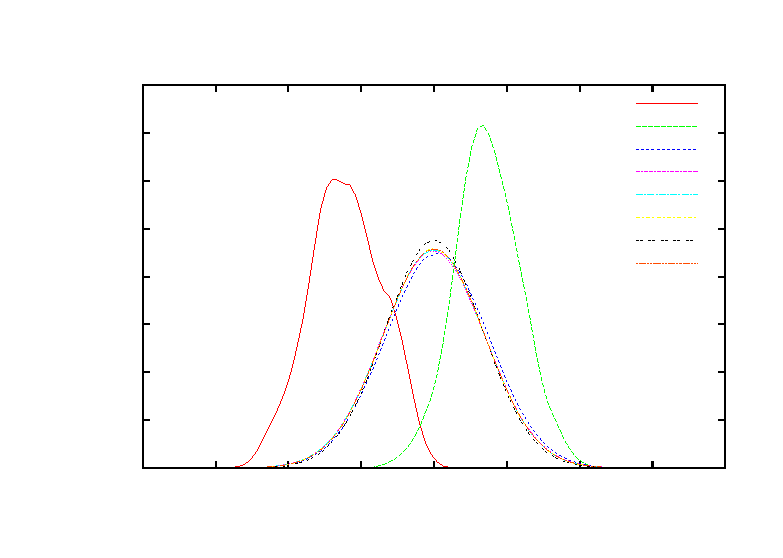
\includegraphics{probability_distributions}}%
    \gplfronttext
  \end{picture}%
\endgroup

\caption{La distribution de probabilité P(x)}
\end{figure}

Nous traçons par la suite la variation de l'énergie moyenne en fonction de $\tau$. Nous remarquons que pour des grandes valeurs de $\tau$ et donc petites valeurs de température $T$, l’énergie moyenne reste autour de la valeur quantique 0.5 (puisque $\hbar=1$). Par contre, pour des petites valeurs de $\tau$, et donc grande $T$, les énergies sont beaucoup plus élevées. 

\begin{figure}[!h]
\centering
% GNUPLOT: LaTeX picture with Postscript
\begingroup
  \makeatletter
  \providecommand\color[2][]{%
    \GenericError{(gnuplot) \space\space\space\@spaces}{%
      Package color not loaded in conjunction with
      terminal option `colourtext'%
    }{See the gnuplot documentation for explanation.%
    }{Either use 'blacktext' in gnuplot or load the package
      color.sty in LaTeX.}%
    \renewcommand\color[2][]{}%
  }%
  \providecommand\includegraphics[2][]{%
    \GenericError{(gnuplot) \space\space\space\@spaces}{%
      Package graphicx or graphics not loaded%
    }{See the gnuplot documentation for explanation.%
    }{The gnuplot epslatex terminal needs graphicx.sty or graphics.sty.}%
    \renewcommand\includegraphics[2][]{}%
  }%
  \providecommand\rotatebox[2]{#2}%
  \@ifundefined{ifGPcolor}{%
    \newif\ifGPcolor
    \GPcolortrue
  }{}%
  \@ifundefined{ifGPblacktext}{%
    \newif\ifGPblacktext
    \GPblacktexttrue
  }{}%
  % define a \g@addto@macro without @ in the name:
  \let\gplgaddtomacro\g@addto@macro
  % define empty templates for all commands taking text:
  \gdef\gplbacktext{}%
  \gdef\gplfronttext{}%
  \makeatother
  \ifGPblacktext
    % no textcolor at all
    \def\colorrgb#1{}%
    \def\colorgray#1{}%
  \else
    % gray or color?
    \ifGPcolor
      \def\colorrgb#1{\color[rgb]{#1}}%
      \def\colorgray#1{\color[gray]{#1}}%
      \expandafter\def\csname LTw\endcsname{\color{white}}%
      \expandafter\def\csname LTb\endcsname{\color{black}}%
      \expandafter\def\csname LTa\endcsname{\color{black}}%
      \expandafter\def\csname LT0\endcsname{\color[rgb]{1,0,0}}%
      \expandafter\def\csname LT1\endcsname{\color[rgb]{0,1,0}}%
      \expandafter\def\csname LT2\endcsname{\color[rgb]{0,0,1}}%
      \expandafter\def\csname LT3\endcsname{\color[rgb]{1,0,1}}%
      \expandafter\def\csname LT4\endcsname{\color[rgb]{0,1,1}}%
      \expandafter\def\csname LT5\endcsname{\color[rgb]{1,1,0}}%
      \expandafter\def\csname LT6\endcsname{\color[rgb]{0,0,0}}%
      \expandafter\def\csname LT7\endcsname{\color[rgb]{1,0.3,0}}%
      \expandafter\def\csname LT8\endcsname{\color[rgb]{0.5,0.5,0.5}}%
    \else
      % gray
      \def\colorrgb#1{\color{black}}%
      \def\colorgray#1{\color[gray]{#1}}%
      \expandafter\def\csname LTw\endcsname{\color{white}}%
      \expandafter\def\csname LTb\endcsname{\color{black}}%
      \expandafter\def\csname LTa\endcsname{\color{black}}%
      \expandafter\def\csname LT0\endcsname{\color{black}}%
      \expandafter\def\csname LT1\endcsname{\color{black}}%
      \expandafter\def\csname LT2\endcsname{\color{black}}%
      \expandafter\def\csname LT3\endcsname{\color{black}}%
      \expandafter\def\csname LT4\endcsname{\color{black}}%
      \expandafter\def\csname LT5\endcsname{\color{black}}%
      \expandafter\def\csname LT6\endcsname{\color{black}}%
      \expandafter\def\csname LT7\endcsname{\color{black}}%
      \expandafter\def\csname LT8\endcsname{\color{black}}%
    \fi
  \fi
  \setlength{\unitlength}{0.0500bp}%
  \begin{picture}(7200.00,5040.00)%
    \gplgaddtomacro\gplbacktext{%
      \csname LTb\endcsname%
      \put(946,934){\makebox(0,0)[r]{\strut{} 0.4}}%
      \put(946,1393){\makebox(0,0)[r]{\strut{} 0.6}}%
      \put(946,1852){\makebox(0,0)[r]{\strut{} 0.8}}%
      \put(946,2312){\makebox(0,0)[r]{\strut{} 1}}%
      \put(946,2771){\makebox(0,0)[r]{\strut{} 1.2}}%
      \put(946,3231){\makebox(0,0)[r]{\strut{} 1.4}}%
      \put(946,3690){\makebox(0,0)[r]{\strut{} 1.6}}%
      \put(946,4149){\makebox(0,0)[r]{\strut{} 1.8}}%
      \put(1135,484){\makebox(0,0){\strut{} 0}}%
      \put(2268,484){\makebox(0,0){\strut{} 200}}%
      \put(3402,484){\makebox(0,0){\strut{} 400}}%
      \put(4536,484){\makebox(0,0){\strut{} 600}}%
      \put(5669,484){\makebox(0,0){\strut{} 800}}%
      \put(6803,484){\makebox(0,0){\strut{} 1000}}%
      \put(176,2541){\rotatebox{-270}{\makebox(0,0){\strut{} Average Energy E}}}%
      \put(3940,154){\makebox(0,0){\strut{}$\tau$}}%
      \put(3940,4709){\makebox(0,0){\strut{}Variation of average energy with $\tau$}}%
    }%
    \gplgaddtomacro\gplfronttext{%
    }%
    \gplbacktext
    \put(0,0){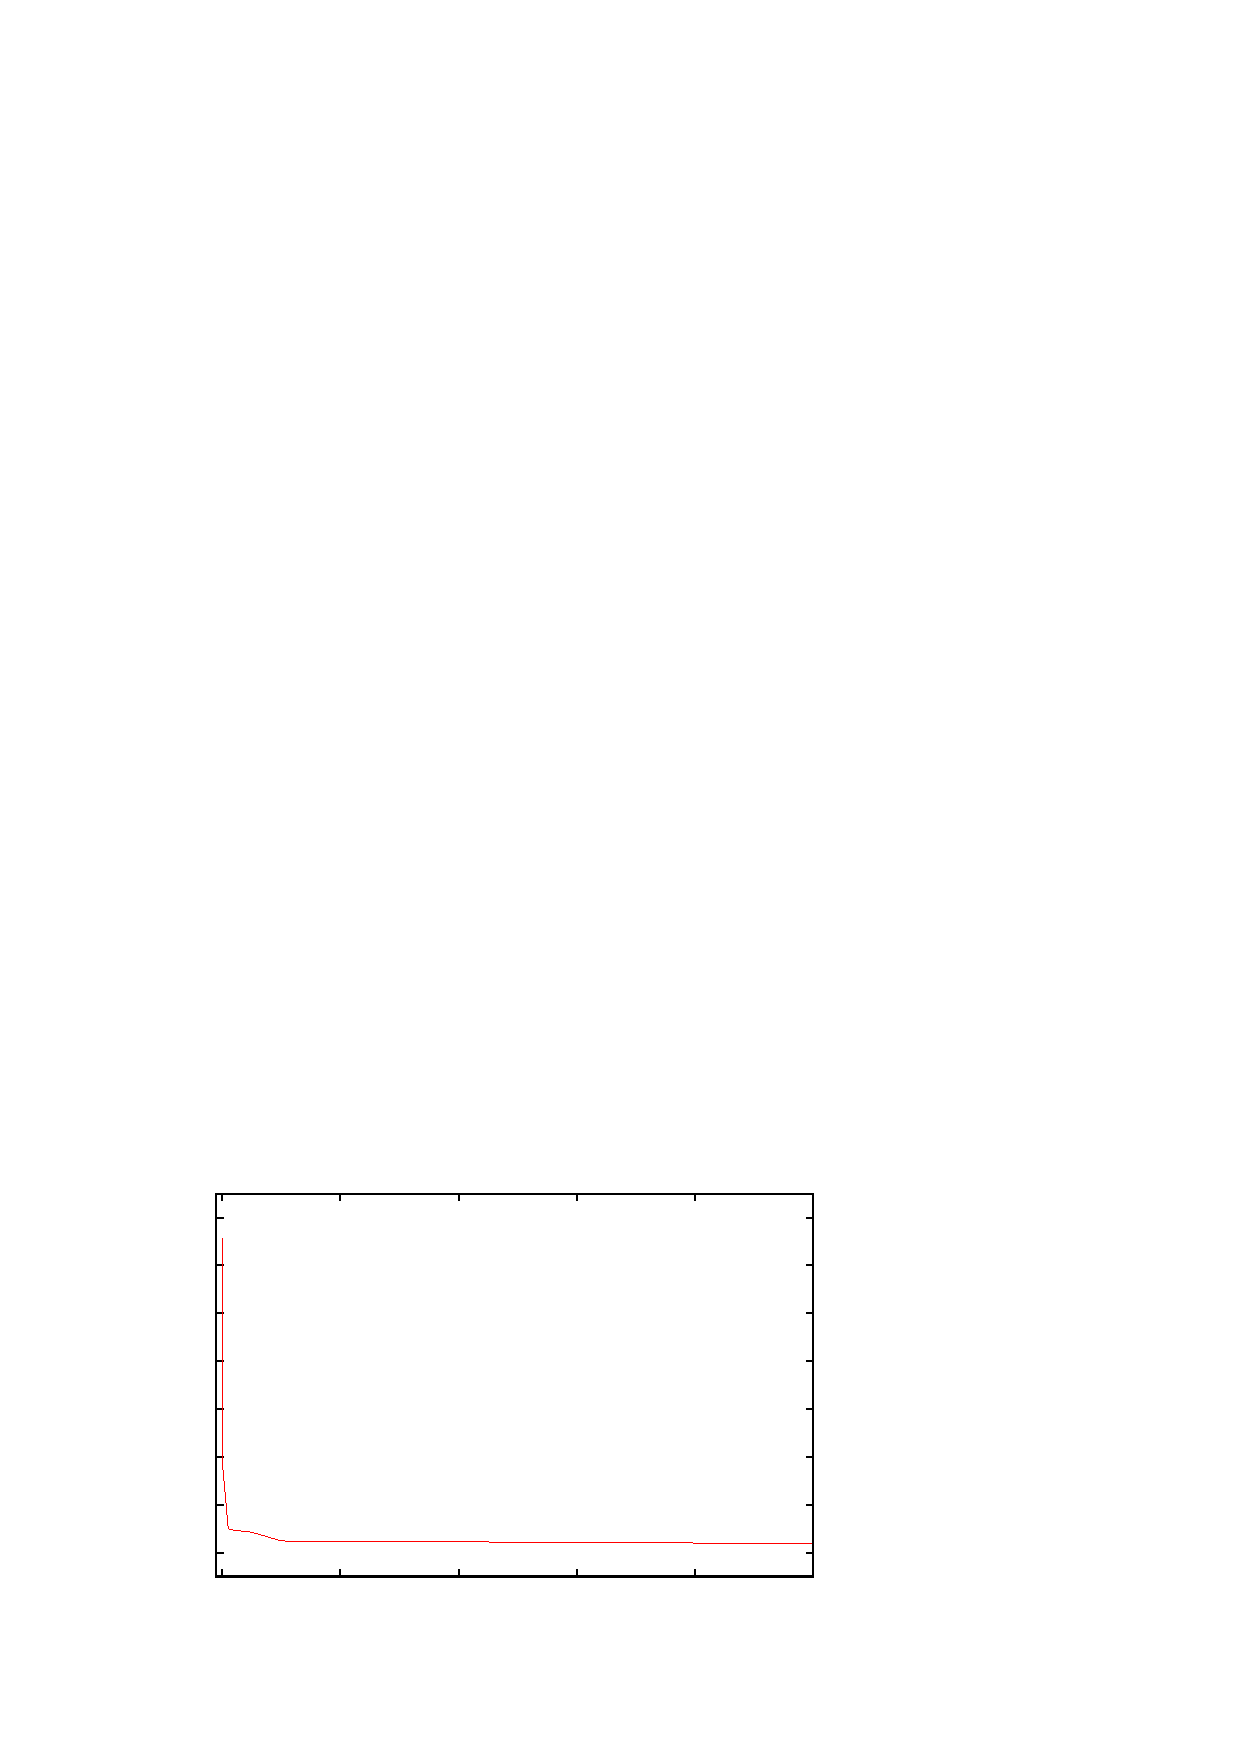
\includegraphics{Energie_moyenne}}%
    \gplfronttext
  \end{picture}%
\endgroup

\caption{Variation de l'énergie moyenne en fonction de $\tau$.}
\end{figure}

\subsubsection{Sampling de Levy} 

Nous savons que l’intégrale de chemin est un outil très puissant. Toutefois, nous avons remarqué lors des simulations que le méthode décrite plus haut n'était pas rapide et qu'il nous fallait beaucoup d’itérations pour trouver les bons chemins. Pour nous affranchir de cette difficulté, nous avons décidé d'utiliser la méthode dite de de "\textbf{Levy Sampling}". De manière générale, le sampling de Lévy généralise les interpolations polynomiales ou trigonométriques en construisant une interpolation stochastique entre deux points $x_0$ et $x_N$. Ainsi, entre deux points de l'intervalle $[\tau_1, \tau_2]$, le chemin reliant $x(\tau_1)$ à $x(\tau_2)$ est l'interpolation stochastique entre ces deux points. De plus le comportement de ce chemin en dehors de cet intervalle n'a pas d'importance. Nous décrivons dans la suite l'utilité de cette méthode et nous proposons à la fin une méthode qui nous permettra de échantillonner les permutations, nécessaires pour traiter des bosons. 

Nous partons d'un point $x_k$ compris entre deux positions fixes $x'$ et $x''$. Nous voulons trouver la probabilité conditionnelle qui le chemin reliant $x'$ et $x''$ passant par le point $x_k$. Pour cela nous avons:

\begin{equation}
\label{proba_levy_1}
\pi^{\mathrm{libre}}(x_k|x',x'') \propto \rho^{\mathrm{libre}}(x', x_k, \Delta_{\tau}') \rho^{\mathrm{libre}}(x_k, x'', \Delta_{tau}'')
\end{equation} 

où les $\rho^{\mathrm{libre}}$ sont les matrices densité correspondant à des particules libres et qui s'écrivent comme : 

\begin{align}
\label{rho_free_levy}
\rho^{\mathrm{libre}}(x', x_k, \Delta_{\tau}') &\propto \mathrm{exp}\Big[ - \frac{(x'-x_k)^2}{2\Delta_{\tau}'} \Big] \\
\rho^{\mathrm{libre}}(x_k, x'', \Delta_{\tau}'') &\propto \mathrm{exp}\Big[ - \frac{(x_k-x'')^2}{2\Delta_{\tau}''} \Big]
\end{align}

En explicitant les termes dans les exponentielles nous trouvons que: 

\begin{align} 
\label{rho_free_levy_2}
\pi^{\mathrm{libre}}(x_k|x',x'') \propto \mathrm{exp}\Big[ - \frac{(x_k - \langle x_k \rangle)^2}{2 \sigma^2} \Big]
\end{align}

où 
\begin{align} 
\langle x_k \rangle &= \frac{\Delta_{\tau}'' x' + \Delta_{\tau}'x''}{\Delta_{\tau}' + \Delta_{\tau}''} \\
\sigma^2 &= \Big(\frac{1}{\Delta_{\tau}''} + \frac{1}{\Delta_{\tau}'}\Big)^{-1}
\end{align}

Nous remarquons alors que cette expression nous permet d'échantillonner les points qui relient deux points donnés $x'$ et $x''$. En particulier, entre $x_0$ et $x_N$, nous pouvons échantillonner le point $x_1$, entre $x_1$ et $x_N$ un point $x_2$, un point $x_3$ etc. jusqu'à la génération de tout le chemin $[x_1 \cdots x_{N-1}]$. Ce méthode nous permet finalement de créer un chemin allant de $x_0$ jusqu'à $x_N$ sans réjection. Concrètement pour générer un chemin entre deux points quelconque, il suffit de échantillonner une distribution gaussienne écart type $\sigma$ pour chaque tranche entre le point de départ $x_0$ et le point d'arrivée $x_N$. 

Dans le cas de l'oscillateur harmonique, nous avons les paramètres suivants: 

\begin{align}
\label{levy_parameters_ho}
\langle x_k \rangle &= \frac{\Gamma_1}{\Gamma_2} \\
\sigma^2 &= \frac{1}{\Gamma_1} \\
\Gamma_1 &= \coth{\Delta_{\tau}'} + \coth{\Delta_{\tau}''} \\
\Gamma_2 &= \frac{x'}{\sinh{\Delta_{\tau}'}} + \frac{x''}{\sinh{\Delta_{tau}''}}
\end{align}

où la probabilité conditionnelle $\pi^{\mathrm{oh}}$ a la même forme que \eqref{rho_free_levy_2}. 

\begin{figure}[!h]
\label{levy_paths}
\centering 
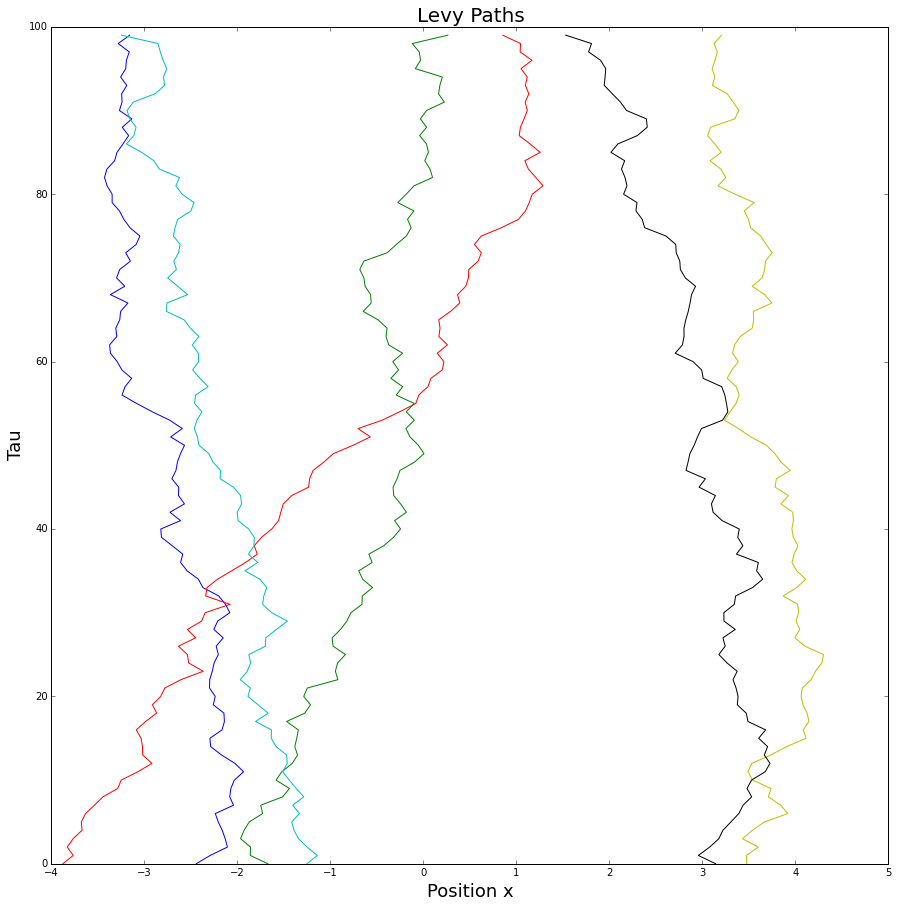
\includegraphics[width=10cm]{levy_paths.png}
\caption{6 chemins de Lévy construits pour différents points de départ.}
\end{figure} 

\subsubsection{Permutation Sampling} 

Nous passons maintenant à l’étape le plus délicate en ce qui concerne la simulations des bosons, c'est-à-dire les permutations. Nous avons déjà évoqué ci-dessus que les bosons doivent avoir une fonction d'onde symétrique. Cela implique que dans les chemins que nous traçons entre deux points $X$ et $X'$ donnés, nous devons prendre en compte toutes les permutations $PX'$ également. Pour un système à $N$ particules, le nombre totale de permutations est très grand (de l'ordre de $N!$). C'est pour cette raison que nous devons trouver un moyen efficace d'échantillonner les permutations. 

Commençons par un cas simple: un système à deux bosons n'intéragissant pas entre eux. Les chemins possible entre deux points fixes pour ces deux particules doivent être interchangeables puisque ce sont des particules indiscernables. Ce type de permutations est très simple: nous pouvons juste échanger les chemins entre les deux particules. 

\begin{figure}[!h]
\label{levy_paths_exchange}
\centering 
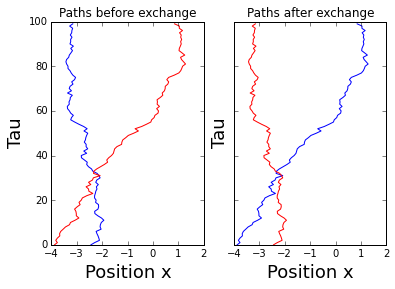
\includegraphics{levy_paths_2.png}
\caption{L'échange entre les particules} 
\end{figure} 

Cependant, nous avons le choix de permuter les positions intermédiaires entre deux points quelconques aussi. C'est ici que nous utilisons la méthode de Lévy afin d’effectuer une permutation entre deux points quelconques sur les chemins des deux particules. Nous le ferons de la façon suivante: 

\begin{enumerate} 
\item 
Tout d'abord nous choisissons deux instants $\tau_1$ et $\tau_2$ entre lesquels nous voulons effectuer un échange. 
\item 
Ensuite, nous supprimons les parties de chemin entre ces deux instants pour les deux particules. Pour les parties restantes en dehors de ces deux instants, nous échangeons les chemins entre les deux particules comme montré plus haut. 
\item 
Une fois échangés, nous créons deux nouveaux sous-chemins entre les instants $\tau_1$ et $\tau_2$ avec la construction de Lévy. La construction est faite comme si les particules étaient libres. Nous avons maintenant deux nouveaux chemins qui ont des positions permutées. 
\item 
Finalement, comment choisissons nous si nous devons accepter ces deux chemins ? Pour cela, nous comparons la différence d'énergie telle qu'elle est décrite en \eqref{energie_trotter} mais cette fois les valeurs de $M$ sont celles qui correspondent aux instants $\tau_1$ et $\tau_2$. Ainsi nous avons une probabilité d'acceptation: 

\begin{equation}
\label{acceptance_levy} 
A(\mathrm{old}\rightarrow \mathrm{new}) = \min\left(1,\frac{\mathrm{exp}(-\beta E_{\mathrm{new}})}{\mathrm{exp}(-\beta E_{\mathrm{old}})}\right)
\end{equation}

où $E_\mathrm{new}$ and $E_\mathrm{old}$ sont des nouvelles et anciennes énergies calculées pour les anciens et les nouveaux chemins selon la formule \eqref{energie_trotter}. 
\end{enumerate}

Cela termine notre algorithme de permutation pour deux particules. Pour plus de particules, nous devons prendre en compte les nombres de voisins de chacune de deux particules qui se trouve à une distance critique donnée. Cela est très important quand nous devons prendre en compte les interactions entre les particules. Mais quand ce n'est pas le cas et que les particules évoluent sans interaction entre elles, nous pouvons tout simplement effectuer l'algorithme décrit ci-dessus. 


\end{document} 